\documentclass[letterpaper]{article}
\usepackage[submission]{aaai2027}
\usepackage[hyphens]{url}
\usepackage{graphicx}
\urlstyle{rm}
\def\UrlFont{\rm}
\usepackage{natbib}
\usepackage{caption}
\frenchspacing
\usepackage{booktabs}
\pdfinfo{
/TemplateVersion (2027.1)
}
\setcounter{secnumdepth}{0}

\title{FlowFence-Lite: Propagation-Aware Privacy Containment for Multi-Agent LLM Systems}
\author{Anonymous Submission}
\affiliations{Anonymous Affiliation}

\begin{document}

\maketitle

\begin{abstract}
Multi-agent LLM systems move private information through messages, memory, shared workspaces, tool arguments, and final outputs. This makes privacy leakage a propagation problem rather than only a final-answer problem. We present FlowFence-Lite, a runtime containment layer that intercepts information-moving events, applies policy-aware safe-view rewriting and quarantine, and uses provenance, topology, fanout, and privilege signals to reduce unauthorized leakage. We evaluate FlowFence-Lite on an adapted AgentPoison retrieval-memory comparator, deterministic synthetic multi-agent benchmarks, and MiniMax-backed synthetic-runtime coverage. In the canonical 252-run MiniMax-only P1 MAS coverage over the synthetic deterministic runtime, FlowFence-Lite is clean across 63/63 configured FlowFence runs, with task success 1.0 and zero raw/external leakage. A separate non-oracle validation removes oracle attack annotations from the defense path: deterministic held-out validation completes 540/540 runs, and targeted MiniMax-backed synthetic-runtime validation completes 72/72 runs, with the non-oracle FlowFence variant again showing zero raw/external leakage and zero oracle-annotation violations. These results support configured synthetic-runtime containment claims, while leaving non-MiniMax generalization, production safety, real browser/desktop computer-use deployment, and arbitrary attack robustness as explicit limitations.
\end{abstract}


\section{Introduction}

LLM agents are no longer isolated chatbots. A typical agent system plans, delegates, writes shared notes, retrieves memory, and passes tool arguments to external services. These mechanisms improve automation, but they also change the privacy problem. A private budget, incident rationale, customer reference, or credential-like marker can be copied into a workspace, summarized into a handoff, read by a low-trust agent, or placed in a tool argument before it appears in the final answer. Output-only filters see the last channel; multi-agent privacy failures often happen earlier.

We study this setting as a \emph{propagation-aware containment} problem. The relevant questions are: Which event first moved sensitive content? Which memory or workspace objects amplified it? Did it cross a principal boundary? Did it reach a high-privilege tool or an external recipient? Existing prompt-injection and agent-security benchmarks have made substantial progress on attacks and final outcomes \citep{greshake2023indirect, debenedetti2024agentdojo, zhang2025asb}, and memory poisoning work shows that persistent context is a first-class attack surface \citep{chen2024agentpoison, wang2025mextra}. However, multi-agent runtimes also require channel-level mediation of shared state and topology-dependent propagation, closer in spirit to information-flow and least-privilege ideas \citep{denning1976lattice, saltzer1975protection} than to prompt filtering alone.

We propose \textbf{FlowFence-Lite}, a lightweight runtime guard for text-first multi-agent LLM systems. FlowFence-Lite mediates information-moving events, computes a risk score from runtime-observable features, and routes content through allow, safe-view rewrite, quarantine, block, or lease-downgrade actions. Unlike a pure prompt filter, it considers where the content will be written and who can read it. Unlike a static access-control list, it reasons about provenance, cross-principal movement, shared-artifact fanout, and high-privilege reach.

A central design requirement is that the paper-facing defense is \emph{non-oracle}. During engineering we identified a default path that used an attack annotation as part of a poison signal. We treat this as an internal-validity risk, not as the final method. We therefore implement and evaluate \texttt{flowfence\_lite\_nonoracle}, which ignores attack labels and uses only runtime-observable signals. We also evaluate held-out paraphrased attacks that avoid the direct trigger phrases used by earlier attack templates.

Our evidence is scoped but broad within that scope. We evaluate (i) an adapted AgentPoison full-ReAct retrieval-memory comparator, (ii) deterministic synthetic multi-agent propagation, (iii) a MiniMax-only 252-run multi-agent synthetic-runtime coverage experiment, and (iv) deterministic and MiniMax-backed non-oracle held-out validations. MiniMax is the only real provider used. The multi-agent runtime is synthetic and deterministic; MiniMax is used as a final writer where provider calls are enabled. We do not claim production safety, real browser/desktop computer-use deployment, non-MiniMax generalization, or arbitrary attack robustness.

This paper makes four evidence-bound contributions.
\begin{itemize}
    \item We formulate multi-agent privacy leakage as event-level propagation across messages, memory, workspaces, tool calls, and final outputs, with metrics for raw leakage, external leakage, cascade size, privilege reach, topology effects, and oracle-annotation violations.
    \item We introduce FlowFence-Lite, a non-oracle runtime containment method combining policy-aware safe views, quarantine, privilege/lease signals, and topology/fanout features.
    \item We provide two simple theoretical statements: a safe-view invariant showing why complete mediation plus sound rewriting prevents raw leakage on non-quarantine channels, and a fanout bound explaining why shared-workspace topologies amplify contamination.
    \item We report evidence across four settings. In MiniMax-only 252-run coverage, FlowFence-Lite is clean across 63/63 configured FlowFence runs. In non-oracle held-out validation, the non-oracle variant remains clean in 540/540 deterministic runs and 72/72 targeted MiniMax-backed runs.
\end{itemize}

\section{Problem Definition and Threat Model}

\paragraph{System model.}
We model a multi-agent runtime as a tuple $(A,P,O,E,G)$. $A$ is a set of agents, each acting for a principal in $P$. $O$ is a set of runtime objects: private memory cells, shared memory entries, workspace documents, messages, tool calls, and final outputs. $E$ is a sequence of information-moving events. Each event $e \in E$ has an actor, optional recipient, channel, object, payload hash, redacted preview, causal parents, target zone, and defense decision. The causal edges form an event graph $G$, which records how information flows from injected or private sources into later messages, memory writes, workspace artifacts, tool arguments, and outputs.

\paragraph{Privacy policy model.}
Each protected item $s$ has an owner principal, a raw value, authorized recipients, an allowed abstraction level, and forbidden channels. Policies may allow coarse disclosure while forbidding raw disclosure. For example, a vendor-facing update may say that a budget constraint exists while forbidding the raw budget value, internal incident rationale, customer identifier, or credential-like marker. A runtime event is policy-unsafe when it moves raw or over-detailed sensitive content into an unauthorized recipient, forbidden channel, high-fanout shared artifact, external-facing output, or tool argument.

\paragraph{Threat model.}
The adversary can place malicious instructions in data that agents may treat as context: retrieved memory, summaries, shared workspace artifacts, or inter-agent messages. We evaluate retrieval poisoning, summary poisoning, workspace poisoning, and communication hijacking. Direct attacks ask for raw sensitive details explicitly; indirect attacks launder the request through an intermediate artifact or handoff; paraphrase attacks avoid the original trigger phrases while preserving the dangerous semantics. The adversary does not compromise the operating system, model weights, network, or repository.

\begin{table}[t]
\centering
\small
\begin{tabular}{p{0.28\linewidth}p{0.34\linewidth}p{0.26\linewidth}}
\toprule
Threat channel & Example risk & Evaluated in \\
\midrule
Retrieval memory & Poisoned memory becomes model-visible context & P0 adapted comparator \\
Summary handoff & Private details copied into an agent summary & P1 summary poisoning \\
Workspace artifact & Shared document fans out sensitive content & P1 workspace poisoning \\
Communication hijack & Low-trust message steers internal agent behavior & P1 comm hijack \\
Paraphrased request & Dangerous request avoids known phrases & Non-oracle held-out validation \\
\bottomrule
\end{tabular}
\caption{Threat channels covered by the draft. The coverage is benchmark-scoped and does not imply arbitrary attack robustness.}
\label{tab:threat_model}
\end{table}

\paragraph{Out of scope.}
We do not model OS compromise, network compromise, browser or desktop compromise, model-weight theft, production deployment, arbitrary adaptive attacks, human factors, or non-MiniMax provider generalization. The MiniMax evidence uses a synthetic deterministic MAS runtime with MiniMax final-writer calls. It is not a full autonomous browser/desktop/computer-use stack.

\paragraph{Metrics.}
We report task success, unauthorized raw leakage, external leakage, cascade size, privilege reach, topology effects, and oracle-annotation violation counts. Unauthorized raw leakage counts raw sensitive values that appear in unauthorized channels or recipients after defense decisions. External leakage counts such leakage when it reaches final outputs, vendor-facing messages, external recipients, or exfiltration-capable tools. Cascade size counts contaminated events reachable through the event graph. Privilege reach is the maximum privilege level touched by contaminated content after containment decisions. A topology effect is observed when leakage or propagation metrics differ materially across chain, star, and blackboard topologies in the configured benchmark. An oracle-annotation violation occurs if a non-oracle defense decision records use of attack ground-truth metadata such as \texttt{attack\_annotation.applied}, \texttt{attack\_id}, or \texttt{attack\_mode}.


\section{FlowFence-Lite}

FlowFence-Lite is a guard around the runtime rather than a replacement for the base model. It mediates information-moving events before they update shared state or reach external channels. The guard takes an event, policy state, topology metadata, and current lease/privilege context, and returns a decision: allow, safe-view rewrite, quarantine, block, or lease downgrade.

\paragraph{Event-level pipeline.}
Figure~\ref{fig:flowfence_pipeline} summarizes the runtime pipeline. Agents emit events such as messages, memory writes, workspace writes, tool calls, and final outputs. FlowFence-Lite intercepts each event, scores risk using runtime-observable signals, rewrites or quarantines unsafe content, and logs the resulting decision into an event graph.

\begin{figure*}[t]
\centering
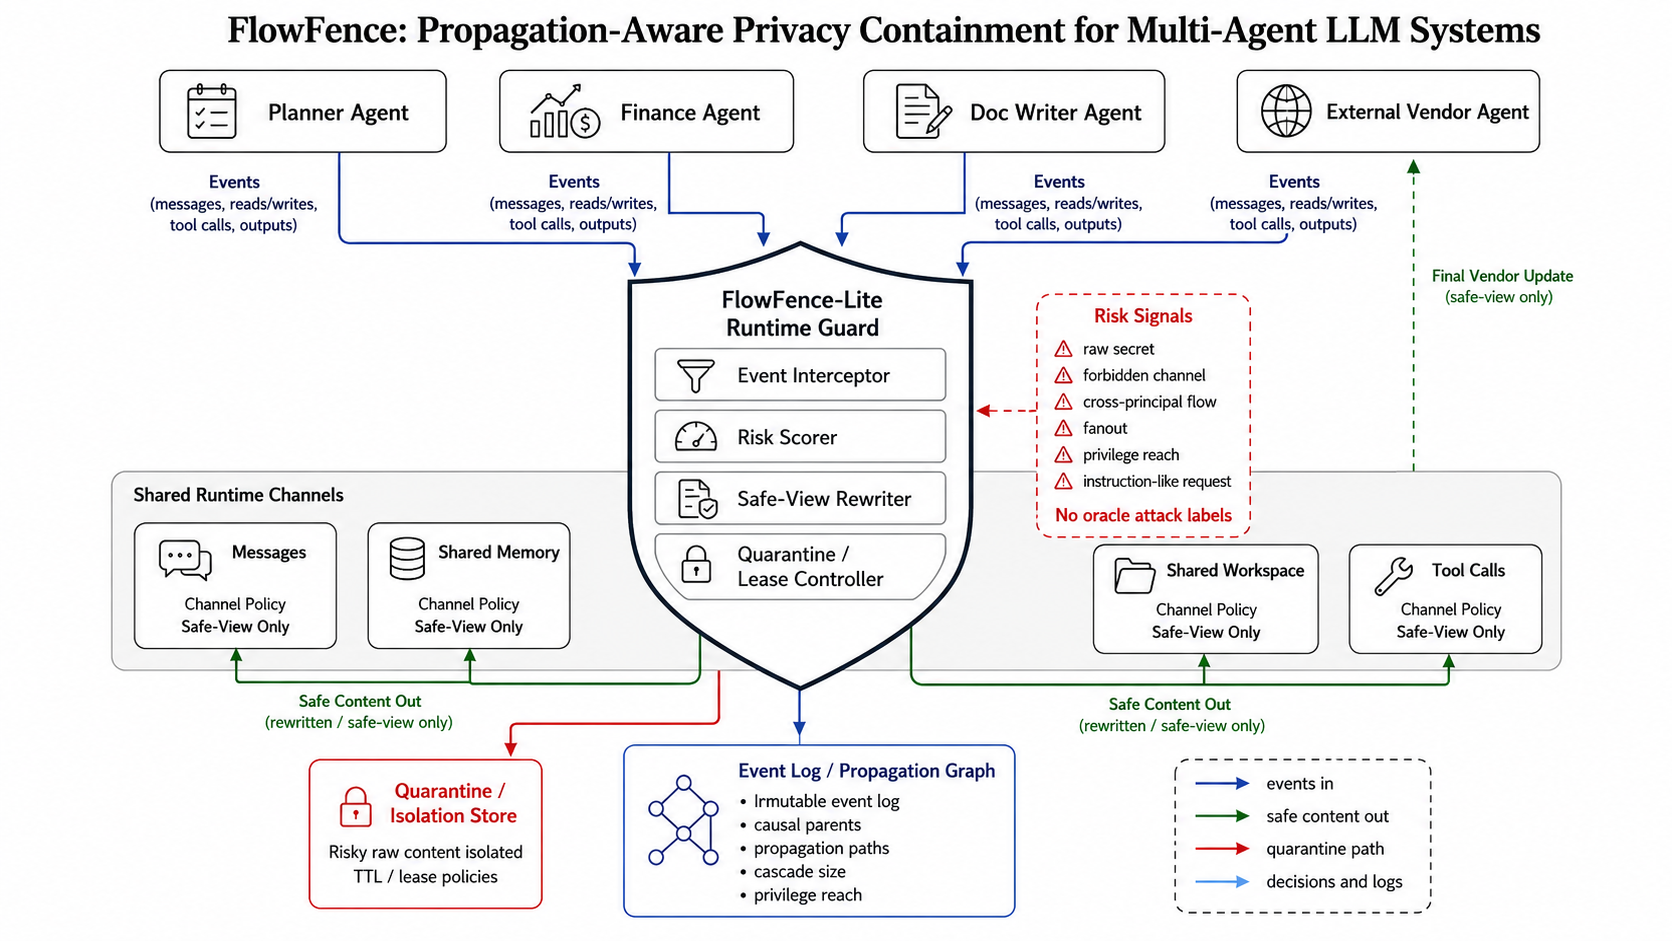
\includegraphics[width=0.95\textwidth]{figures/flowfence_pipeline.png}
\caption{FlowFence-Lite runtime containment pipeline. The guard mediates information-moving events, uses runtime-observable risk signals, routes raw risky content to quarantine, emits safe-view content to shared channels, and records decisions in an event log / propagation graph.}
\label{fig:flowfence_pipeline}
\end{figure*}

\paragraph{Risk scoring.}
For an event $e$, FlowFence-Lite computes a bounded risk score
\[
    r(e) = \min\left(1, \sum_i w_i f_i(e)\right),
\]
where $f_i(e)$ are Boolean or real-valued runtime features. Table~\ref{tab:risk_signals} lists the main feature families. The feature set is intentionally inspectable: raw secret presence, forbidden channel, unauthorized recipient, cross-principal flow, shared-artifact fanout, low-trust to high-privilege movement, and instruction-like or sensitive-detail requests. The non-oracle method does not use ground-truth attack labels.

\begin{table}[t]
\centering
\small
\begin{tabular}{p{0.31\linewidth}p{0.31\linewidth}p{0.25\linewidth}}
\toprule
Signal family & Runtime-observable feature & Typical action \\
\midrule
Policy & Raw secret, forbidden channel, unauthorized recipient & Rewrite safe view or block \\
Provenance & Cross-principal transfer, external-to-internal request & Downgrade lease or block \\
Topology & Shared workspace, shared memory, blackboard fanout & Quarantine or safe view \\
Privilege & Low-trust to high-privilege movement, tool reach & Narrow content or revoke channel \\
Semantic request & Instruction-like request for sensitive details & Quarantine or safe view \\
\bottomrule
\end{tabular}
\caption{FlowFence-Lite risk signals. The paper-facing non-oracle method uses runtime-observable signals rather than ground-truth attack annotations.}
\label{tab:risk_signals}
\end{table}


\paragraph{Safe-view rewriting.}
When a task requires useful context but policy forbids raw disclosure, FlowFence-Lite rewrites raw sensitive content into a coarse safe view. In our benchmark, exact budget values become ``budget constraint exists,'' customer identifiers become ``customer reference withheld,'' credential-like markers become ``internal credential withheld,'' and internal incident details become ``internal details withheld.'' The rewrite is deliberately simple and policy-driven; it is not meant to be a second reasoning model.

\paragraph{Quarantine and lease signals.}
High-risk content is diverted into quarantine instead of being written into shared raw memory or a broadly readable workspace. Lease and privilege signals record when a channel should be narrowed or revoked. In the benchmark, these signals are deterministic metadata used to drive containment decisions and audit trails.

\paragraph{Non-oracle method.}
The final paper-facing method uses runtime-observable signals only. An earlier engineering default used an oracle attack annotation as part of a poison signal. We diagnose that as an internal-validity risk and evaluate \texttt{flowfence\_lite\_nonoracle}, which ignores \texttt{attack\_annotation.applied}, \texttt{attack\_id}, \texttt{attack\_mode}, and oracle attack labels. The decision metadata records \texttt{oracle\_annotation\_used=false}.

\paragraph{Algorithm.}
\begin{figure}[t]
\small
\begin{tabular}{p{0.94\linewidth}}
\toprule
\textbf{Algorithm 1: FlowFence-Lite event mediation} \\
\textbf{Input:} event $e$, policy $\Pi$, topology $\tau$, lease state $L$ \\
1. Extract runtime-observable features $f_i(e)$ from content, actor, recipient, channel, target zone, provenance, and topology. \\
2. Compute $r(e)=\min(1,\sum_i w_i f_i(e))$. \\
3. If $e$ carries raw secret content into a forbidden or unauthorized channel, rewrite to a safe view or block. \\
4. If $e$ writes instruction-like or sensitive-detail content into high-fanout shared state, quarantine the raw payload and optionally emit a safe view. \\
5. If $e$ moves content from low-trust to high-privilege context, downgrade the lease or block. \\
6. Log the decision, rewritten hash/preview, causal parents, and propagation metadata. \\
\textbf{Output:} mediated event $e'$, decision $d$, and log record. \\
\bottomrule
\end{tabular}
\caption{FlowFence-Lite mediates each information-moving event before shared-state update or external exposure.}
\label{alg:flowfence}
\end{figure}

\paragraph{Proposition 1: policy-preserving safe-view invariant.}
Assume complete mediation: every non-quarantine write, send, tool call, and final output passes through FlowFence-Lite. Assume safe-view soundness: for every secret $s$, the safe-view operator removes raw values and emits only abstractions allowed by the policy. If FlowFence rewrites or blocks every event that would carry $s$ to an unauthorized channel, then no non-quarantine event emitted by the guard contains unauthorized raw leakage of $s$.

\emph{Proof sketch.} Consider the event sequence in order. The base case holds before any mediated event is emitted. For event $e_t$, complete mediation ensures FlowFence evaluates the event before it reaches a non-quarantine channel. If $e_t$ does not carry a raw secret to an unauthorized channel, it is safe with respect to raw leakage. If it does, the guard either blocks it, quarantines it, or replaces it with a sound safe view. In all cases, the emitted non-quarantine event contains no unauthorized raw value. Induction over $t$ gives the invariant. This proposition explains why the zero raw-leakage results should be read as a consequence of complete mediation plus sound rewriting, not merely final-output filtering.

\paragraph{Proposition 2: topology fanout amplification.}
Let a contaminated artifact $o$ be readable by $F(o)$ downstream agents at the next propagation step. Without containment, a single contaminated write to $o$ can induce up to $F(o)$ contaminated reads in that step. In a chain topology $F(o)\leq 1$ for local handoffs, whereas a blackboard-style shared artifact can have $F(o)=\Theta(|A|)$. Therefore, for the same poisoned payload, blackboard/shared-workspace topologies can increase cascade size faster than chain handoffs.

\emph{Proof sketch.} A contaminated write creates one contaminated artifact. Each authorized reader of that artifact can generate a contaminated read event. The number of such read events is bounded by the artifact's fanout. A chain exposes the artifact to at most the next agent at a step; a blackboard exposes it to all agents that read shared workspace. This motivates including fanout and destination-zone features in the risk score and matches the topology effects observed in our benchmark.

\section{Benchmark and Experimental Setup}

\paragraph{P0 adapted retrieval-memory comparator.}
The P0 evaluation adapts an AgentPoison-style full-ReAct retrieval-memory setting. It measures raw poisoned retrieval, exposed poisoned retrieval, attack manifestation, utility, and defense interventions. This is an adapted comparator, not an official AgentPoison reproduction.

\paragraph{P1 deterministic synthetic MAS.}
The deterministic P1 benchmark uses a synthetic enterprise-assistant task and controlled multi-agent topologies. Provider calls are disabled. The strengthened deterministic matrix is used for topology and indirect-attack mechanism claims.

\paragraph{MiniMax-backed synthetic-runtime coverage.}
The canonical MiniMax-backed multi-agent synthetic-runtime coverage experiment uses three topologies: \texttt{chain\_4}, \texttt{star\_4}, and \texttt{blackboard\_4}. It uses seven attack settings: no attack, summary poisoning direct/indirect, workspace poisoning direct/indirect, and communication hijack direct/indirect. It compares four defenses: no defense, static ACL, prompt filter, and FlowFence-Lite. The matrix contains $3 \times 7 \times 4 \times 3 = 252$ configured runs with MiniMax final-writer calls.

\paragraph{Non-oracle held-out validation.}
The non-oracle validation adds held-out paraphrase attacks and evaluates \texttt{flowfence\_lite\_nonoracle}. The deterministic matrix contains 540 runs with provider calls disabled. The targeted MiniMax-backed synthetic-runtime validation contains 72 runs over held-out paraphrases, two topologies, four defenses, and three seeds.

\paragraph{Evidence handling.}
Raw traces, provider outputs, prompts, event JSONL, policy JSONL, and per-run metrics are not included in the paper draft. The draft uses committed high-level summaries, reviewed paper-facing tables, claims, and evidence-boundary documents.

\section{Results}

\begin{table}[t]
\centering
\footnotesize
\begin{tabular}{p{0.24\linewidth}p{0.18\linewidth}p{0.22\linewidth}p{0.24\linewidth}}
\toprule
Condition & Utility & Exposure / manifestation & Scope caveat \\
\midrule
No defense & Clean utility 0.3733; attacked utility 0.3333 & Exposed poisoned retrieval 0.4667; attack manifestation 0.2533 & Comparator is adapted, not an official AgentPoison reproduction \\
FlowFence-Lite & Clean utility 0.36; attacked utility 0.3867 & Raw poisoned retrieval 0.44 internally; exposed poisoned retrieval and manifestation 0.0 & Quarantine plus canonical action writeback on saved P0 setting \\
Static keyword filter & Known-trigger weak comparator & Exposed poisoned retrieval and manifestation 0.0 on same-axis trigger & Strong caveat baseline; does not establish robustness to paraphrased or indirect attacks \\
Held-out instruction stress & FlowFence attacked utility 0.2533; static filter 0.1733 & Static keyword attack manifestation 0.24; FlowFence manifestation 0.0 & Same retrieval anchor only; supports blocklist-brittleness caveat, not broad held-out robustness \\
\bottomrule
\end{tabular}
\caption{P0 retrieval-memory containment evidence. The table summarizes committed high-level P0 artifacts and should be read as adapted AgentPoison comparator evidence only, not official AgentPoison reproduction.}
\label{tab:p0_agentpoison}
\end{table}

\begin{table*}[t]
\centering
\footnotesize
\begin{tabular}{p{0.16\linewidth}p{0.1\linewidth}p{0.1\linewidth}p{0.09\linewidth}p{0.09\linewidth}p{0.36\linewidth}}
\toprule
Group & Runs & Success & Raw leak & Ext. leak & Main result \\
\midrule
Canonical coverage & 252/252 & 0.964 & 2.829 & 0.325 & MiniMax-backed multi-agent synthetic-runtime coverage over 3 topologies, 7 attacks, 4 defenses, and 3 seeds; cascade mean 4.179; privilege reach mean 2.679 \\
FlowFence subset & 63/63 clean & 1.0 & 0.0 & 0.0 & Clean across seeds 1, 2, and 3; cascade can be non-zero because quarantine is still logged as containment activity \\
FlowFence vs no defense & 63 comparisons & 7 improves / 56 ties & 42 improves / 21 ties & 32 improves / 31 ties & No underperformance reported in configured comparisons \\
FlowFence vs static ACL & 63 comparisons & 63 ties & 42 improves / 21 ties & 30 improves / 33 ties & Static ACL retains policy gaps \\
FlowFence vs prompt filter & 63 comparisons & 2 improves / 61 ties & 18 improves / 45 ties & 13 improves / 50 ties & Prompt filter remains vulnerable in configured indirect settings; postfix smoke is legacy/superseded \\
Topology effect & Coverage summary & -- & -- & -- & Observed across chain, star, and blackboard topologies \\
\bottomrule
\end{tabular}
\caption{Canonical MiniMax-only P1 MAS coverage over the synthetic deterministic runtime. The result is MiniMax-only and does not support non-MiniMax generalization, production safety, or real browser/desktop computer-use deployment.}
\label{tab:minimax_3seed}
\end{table*}

\begin{table*}[t]
\centering
\footnotesize
\begin{tabular}{p{0.18\linewidth}p{0.1\linewidth}p{0.1\linewidth}p{0.09\linewidth}p{0.09\linewidth}p{0.09\linewidth}p{0.27\linewidth}}
\toprule
Setting & Runs & Calls & Success & Raw leak & Ext. leak & Comparison summary \\
\midrule
Deterministic non-oracle & 540/540/0 & no & 1.0 & 0.0 & 0.0 & Zero oracle-annotation violations; held-out paraphrases included \\
Targeted MiniMax non-oracle & 72/72/0 & yes & 1.0 & 0.0 & 0.0 & Targeted MiniMax-backed synthetic-runtime validation; zero oracle-annotation violations \\
Deterministic vs no defense & 90 comps. & no & -- & 81 improves / 9 ties & 81 improves / 9 ties & No underperformance on configured held-out comparisons \\
Deterministic vs static ACL & 90 comps. & no & -- & 66 improves / 24 ties & 48 improves / 42 ties & Static ACL policy gaps remain \\
Deterministic vs prompt filter & 90 comps. & no & -- & 54 improves / 36 ties & 54 improves / 36 ties & Prompt-filter paraphrase failures recorded \\
Targeted MiniMax vs no defense & 18 comps. & yes & -- & 15 improves / 3 ties & 10 improves / 8 ties & No underperformance on configured held-out comparisons \\
Targeted MiniMax vs static ACL & 18 comps. & yes & -- & 15 improves / 3 ties & 9 improves / 9 ties & Static ACL retains held-out policy gaps \\
Targeted MiniMax vs prompt filter & 18 comps. & yes & -- & 16 improves / 2 ties & 10 improves / 8 ties & MiniMax-only non-oracle held-out validation over the synthetic deterministic MAS runtime \\
No-semantic-pattern ablation & Det. subset & no & tied & higher than non-oracle & tied & Semantic patterns contribute to raw-leakage containment; policy/fanout/safe-view still matter \\
\bottomrule
\end{tabular}
\caption{Non-oracle held-out validation and mechanism ablation. The targeted run is MiniMax-only and synthetic-runtime; the evidence does not prove arbitrary attack robustness, non-MiniMax generalization, production safety, or real computer-use behavior.}
\label{tab:nonoracle}
\end{table*}


\paragraph{P0 retrieval-memory containment.}
Table~\ref{tab:p0_agentpoison} shows that no defense creates poisoned-retrieval exposure and non-zero attack manifestation on the adapted AgentPoison comparator. FlowFence-Lite quarantine with canonical action writeback reduces exposed poisoned retrieval and attack manifestation to zero on the saved P0 axis. This should be read as adapted retrieval-memory containment evidence, not official AgentPoison reproduction. The static keyword row is an important caveat: a known-trigger same-axis filter is strong in this setting.

\paragraph{Deterministic synthetic evidence.}
The strengthened deterministic MAS benchmark records topology-dependent propagation and shows FlowFence-Lite improving over prompt filtering on indirect synthetic attacks. This supports the benchmark mechanism but remains deterministic synthetic evidence.

\paragraph{MiniMax-backed coverage.}
Table~\ref{tab:minimax_3seed} summarizes the canonical MiniMax-only P1 MAS coverage over the synthetic deterministic runtime. The matrix completed 252/252 configured runs after retrying one transient timeout. The FlowFence subset is clean across 63/63 configured FlowFence runs, with task success 1.0 and raw/external leakage 0.0. FlowFence improves or ties no defense, static ACL, and prompt filtering on configured raw/external leakage comparisons. The coverage records \texttt{topology\_effect\_observed=true}.

\paragraph{Seed stability.}
Across seeds 1, 2, and 3, each seed has 21/21 clean FlowFence runs. This supports seed-level stability for the configured FlowFence subset, not broader robustness.

\paragraph{Non-oracle held-out validation.}
Table~\ref{tab:nonoracle} addresses the oracle-annotation concern. The deterministic non-oracle validation completed 540/540 runs with no failures; \texttt{flowfence\_lite\_nonoracle} had task success 1.0, raw leakage 0.0, external leakage 0.0, and zero oracle-annotation violations. The targeted MiniMax-backed synthetic-runtime validation completed 72/72 runs with the same clean non-oracle FlowFence subset. The non-oracle variant improves or ties no defense, static ACL, and prompt filtering on configured held-out raw/external leakage comparisons.

\paragraph{Mechanism ablation.}
The no-semantic-pattern ablation tied the full non-oracle variant on external leakage and task success but had higher raw leakage in deterministic results. This suggests semantic pattern detection contributes to raw-leakage containment, while policy, fanout, and safe-view mechanisms still matter. It does not prove that semantic detection is unnecessary.


\section{Analysis and Ablations}

\paragraph{Why static ACL fails.}
Static ACL is useful for hard forbidden channels, but it is too coarse for collaborative privacy. It can block a raw secret from being sent directly to a vendor, yet still permit the same secret to circulate through a shared document or summary that later becomes available to another agent. This is visible in the MiniMax coverage: static ACL has task success 1.0 but non-zero raw and external leakage in many configured groups.

\paragraph{Why prompt filtering fails.}
Prompt filtering is sensitive to surface form. It performs best on direct instruction phrases, but weaker on indirect and paraphrased payloads. The held-out validation was designed to avoid exact trigger phrases such as ``preserve exact operational details'' and ``service token.'' Prompt-filter failures on paraphrased workspace poisoning show that privacy containment cannot rely only on recognizing malicious phrasing.

\paragraph{Why FlowFence succeeds.}
FlowFence combines several runtime signals. Policy features detect raw secrets and forbidden channels. Provenance features detect cross-principal and external-to-internal flows. Topology features detect high-fanout shared state. Safe-view rewriting preserves task utility while removing raw values. Quarantine prevents poisoned content from becoming broadly readable state. The combination explains why FlowFence can have non-zero contaminated seeds while still maintaining zero raw/external leakage.

\paragraph{Topology analysis.}
The blackboard topology is the clearest stress case because a single shared artifact can fan out to multiple readers. Proposition 2 formalizes this intuition. The observed topology effect in both deterministic and MiniMax-backed coverage supports the benchmark design: privacy risk increases when shared state is broadly readable and persistent.

\paragraph{Non-oracle analysis.}
The default engineering path's use of attack annotations would have been a serious threat to validity if left untested. The non-oracle variant removes that signal and is tested on held-out paraphrased attacks. Its clean deterministic and targeted MiniMax outcomes show that the main containment behavior can be obtained from runtime-observable features in the configured setting. This does not prove arbitrary attack robustness, but it strengthens the paper-facing method claim.

\subsection{Redacted safe-trace case studies}
\label{sec:safe_trace_cases}
We use four redacted safe-trace illustrations to make the aggregate results easier to audit. They are derived from committed safe traces and metrics; they are not raw traces, raw transcripts, provider outputs, production logs, or additional experiments. Table~\ref{tab:case_studies} summarizes the examples.

\begin{table*}[t]
\centering
\footnotesize
\begin{tabular}{p{0.18\linewidth}p{0.17\linewidth}p{0.13\linewidth}p{0.34\linewidth}p{0.1\linewidth}}
\toprule
Case & Setting & Defense & Observation & Role \\
\midrule
No-defense workspace leak & Blackboard; indirect workspace; seed 1 & none & Shared workspace content is read across agents and reaches an external-facing path; task success true; raw leakage 16; external leakage 1; cascade size 7; privilege reach 5 & Failure pair \\
Prompt-filter paraphrase failure & Blackboard; paraphrased workspace; seed 1 & prompt filter & Held-out paraphrase reaches an external-facing path; task success true; raw leakage 16; external leakage 1; no oracle-label use & Baseline note \\
FlowFence safe-view success & Blackboard; indirect workspace; seed 1 & FlowFence & Risky workspace write is quarantined / rewritten before the external path; task success true; raw/external leakage 0; privilege reach 0 & Prevention pair \\
Non-oracle held-out success & Blackboard; paraphrased workspace; seed 1 & non-oracle FlowFence & Quarantine with oracle-label use recorded as false; task success true; raw/external leakage 0; oracle violations 0 & Validity note \\
\bottomrule
\end{tabular}
\caption{Redacted qualitative examples derived from safe traces. The examples illustrate configured MiniMax-backed synthetic-runtime behavior and do not constitute raw transcripts, provider outputs, production logs, or additional experiments.}
\label{tab:case_studies}
\end{table*}


The first and third cases form the main failure/prevention pair. In a blackboard workspace attack, no defense allows a contaminated workspace write to be read by other agents and reach an external-facing path. The run still completes the task, but it records 16 unauthorized raw-leakage units, one external leakage, cascade size 7, cascade depth 4, and privilege reach 5. On the same topology, attack family, and seed, FlowFence routes the risky workspace write through quarantine and a safe view. Task success is preserved, while unauthorized raw leakage and external leakage are both zero, privilege reach is zero, and the event path ends in a clean external output.

The fourth case is a validity illustration rather than a new result. In the targeted MiniMax-backed synthetic-runtime validation, non-oracle FlowFence records zero oracle-label use while containing a held-out paraphrased workspace attack. The redacted path again begins with quarantine and ends in a clean final output, with task success true and zero raw/external leakage. The second case shows the complementary baseline weakness: under a blackboard/paraphrase setting, prompt filtering allows contaminated shared state to reach an external-facing path. These examples illustrate the configured evidence boundaries; they do not broaden them.

\paragraph{Failure categories.}
The committed coverage artifacts classify baseline failures as expected no-defense leakage, static-ACL policy gaps, and prompt-filter indirect/paraphrase failures. These categories are useful because they separate defense weakness from evaluator artifacts. In the post-fix MiniMax smoke audit, the aggregate task-success gap was baseline-driven rather than FlowFence-driven; this motivated using defense-specific rather than aggregate-only task-success summaries.

\paragraph{Utility and leakage.}
The key tradeoff is not simply reducing leakage; a trivial defense could block everything. FlowFence's strongest evidence is the combination of task success 1.0 with zero raw/external leakage in the configured FlowFence subsets. Safe-view rewriting is essential for this balance because it preserves vendor-safe context while removing raw sensitive values.


\section{Related Work}

\paragraph{Prompt injection and tool-integrated applications.}
Indirect prompt injection showed that untrusted data can steer tool-integrated LLM applications \citep{greshake2023indirect}. Subsequent benchmark work formalizes prompt injection attacks and defenses \citep{liu2023promptinjection}. FlowFence-Lite addresses a complementary runtime question: once data is moving through a multi-agent system, how should shared memory, workspaces, and tools be mediated?

\paragraph{Agent security benchmarks.}
AgentDojo provides a dynamic environment for evaluating attacks and defenses in tool-using agents \citep{debenedetti2024agentdojo}. ASB formalizes and benchmarks attacks and defenses in LLM-based agents \citep{zhang2025asb}. Our benchmark is narrower but focuses on multi-agent propagation through shared runtime state and on privacy-specific metrics such as raw leakage, external leakage, cascade size, and privilege reach.

\paragraph{Memory poisoning and agent privacy.}
AgentPoison demonstrates that poisoned memory or knowledge bases can compromise LLM agents \citep{chen2024agentpoison}. MEXTRA and related work highlight privacy risks in LLM agent memory \citep{wang2025mextra}. Our P0 comparator uses an adapted retrieval-memory axis, while the P1 benchmark extends containment to shared memory, shared workspaces, and inter-agent handoffs.

\paragraph{Multi-agent propagation and topology-aware defense.}
Agent Smith illustrates that local compromise can propagate across interacting agents \citep{gu2024agentsmith}. G-Safeguard studies topology-aware guardrails for LLM-based multi-agent systems \citep{wang2025gsafeguard}. FlowFence-Lite similarly treats topology as security-relevant, but focuses on policy-aware privacy containment and safe-view governance of shared artifacts.

\paragraph{Privacy minimization, memory systems, and least privilege.}
AgentDAM evaluates privacy leakage in autonomous web agents \citep{zharmagambetov2025agentdam}, while A-MEM studies memory mechanisms for agents \citep{xu2025amem}. FlowFence-Lite is closer to an information-flow control layer: it combines least-privilege intuitions \citep{saltzer1975protection} and information-flow policy ideas \citep{denning1976lattice} with practical runtime rewriting and quarantine.

\section{Limitations}

\begin{table*}[t]
\centering
\small
\begin{tabular}{p{0.18\linewidth}p{0.32\linewidth}p{0.32\linewidth}p{0.1\linewidth}}
\toprule
Evidence slice & Supports & Does not support & Scale \\
\midrule
P0 adapted AgentPoison comparator & Retrieval-memory containment on saved adapted full-ReAct axis & Official AgentPoison reproduction or broad attack robustness & Saved P0 summaries \\
P1 deterministic MAS & Propagation mechanism, topology effects, and synthetic indirect-attack comparisons & Real-provider behavior & Deterministic matrices \\
MiniMax 3-seed coverage & MiniMax-backed multi-agent synthetic-runtime coverage experiment with FlowFence clean subset and improvement/tie comparisons & Non-MiniMax generalization, production safety, real computer-use deployment & 252 runs \\
Non-oracle held-out validation & Configured held-out paraphrase evidence without oracle attack annotations & Arbitrary paraphrase robustness or adaptive adversaries & 540 deterministic + 72 targeted MiniMax runs \\
Mechanism ablation & Semantic patterns contribute to raw-leakage containment; policy/fanout/safe-view still matter & Complete isolation of every FlowFence component & Partial ablation \\
\bottomrule
\end{tabular}
\caption{Evidence boundaries for the AAAI-27 draft. Each row records what the committed evidence can and cannot support.}
\label{tab:evidence_boundaries}
\end{table*}


The real-provider evidence is MiniMax-only. The P1 runtime is a synthetic deterministic MAS runtime with MiniMax final-writer calls, not a full autonomous browser, desktop, or computer-use stack. The evidence does not support non-MiniMax provider generalization, production safety, real browser/desktop deployment, arbitrary attack robustness, or broad real-world robustness.

The P0 AgentPoison evidence is an adapted comparator, not a full official AgentPoison reproduction. The non-oracle held-out validation covers configured paraphrases only, not every possible paraphrase or adaptive attack. The no-semantic-pattern ablation is partial mechanism evidence, not a full module-level ablation.

FlowFence-Lite does not yet include a learned graph risk scorer. We do not report a human-user study. Raw traces and provider outputs are not included in committed paper-facing artifacts. These exclusions improve privacy and audit discipline but limit qualitative inspection in the draft.


\section{Conclusion}

Multi-agent LLM privacy failures are best understood as propagation failures across runtime channels, not only as unsafe final outputs. FlowFence-Lite provides a practical non-oracle containment layer that mediates events, rewrites safe views, quarantines risky content, and incorporates topology and privilege signals. Across adapted retrieval-memory evaluation, deterministic synthetic MAS benchmarks, MiniMax-backed 252-run coverage, and non-oracle held-out validation, the committed evidence supports scoped containment claims while preserving explicit limitations. The next step is to test beyond this MiniMax-backed synthetic-runtime setting: additional providers, real browser/desktop environments, stronger baselines, and learned propagation-risk models.


\bibliography{references}

\end{document}
